
This section describes scenario runs using ElecSIM. Here, we vary the carbon tax and either grow or reduce total electricity demand. This was done to observe the effects of carbon tax policy on long-term investment.

We assume that carbon tax is set by the government, and not subject to market forces such as the EU Emissions Trading Scheme \cite{Council2016}.

We run 16 different scenarios 8 times each, with demand increasing by 1\% per year and decreasing by 1\% a year with varying carbon prices. In this section we explore a decreasing demand of 1\% a year. We chose this due to the increasing efficiency of homes, industry and technology, and due to the recent trend in the UK. Demand, however, does not have a large effect on the optimum carbon price.

Table \ref{table:scenario_statistics}, in the appendix, displays the summary statistic of each run in full.

It can be seen from Figure \ref{fig:demand99carbon10} that a carbon tax of \textsterling10 per year does little to influence investment in low-carbon, renewable technology. With traditional, fossil fuel based generation, providing the majority of supply throughout each year. However, there is an increase in renewable technology over the years, starting from mean 15.85\% market share in the year range 2019-2029, to 24.38\% in the year range 2039-2050. However, a similar increase of renewable energy with a carbon tax of \textsterling0 can be seen, albeit at a lower mean by the year range 2039-2050 (22.29\%).

The UK Government BEIS have predicted a carbon tax increasing from \textsterling18 to \textsterling200 by 2050. With carbon price ncreasingly linearly from 2030 to 2050. This models the EU ETS carbon price. We have approximated these assumptions in Figure \ref{fig:demand99carbon18} and modelled the results. Interestingly, the results show only a slight increase in low-carbon supply over the \textsterling20 carbon tax energy mix. This demonstrates the importance of long-term modelling, and understanding the long-term impacts that can result due to today's decisions.

It is hypothesised that a lower carbon tax early on changes the market dynamics for years to come, due to certain price structures, and therefore it takes a long time for renewable energy to recover.

Figure \ref{fig:demand99carbon40} shows that a carbon tax of \textsterling40 is sufficient in moving demand towards a low-carbon economy, with backup fossil fuel generators.

However, by referring to Figure \ref{fig:demand99carbon70} it can be seen that to have 100\% renewable, a carbon price of \textsterling70 is required. 

\begin{figure}[h]
	\begin{center}
		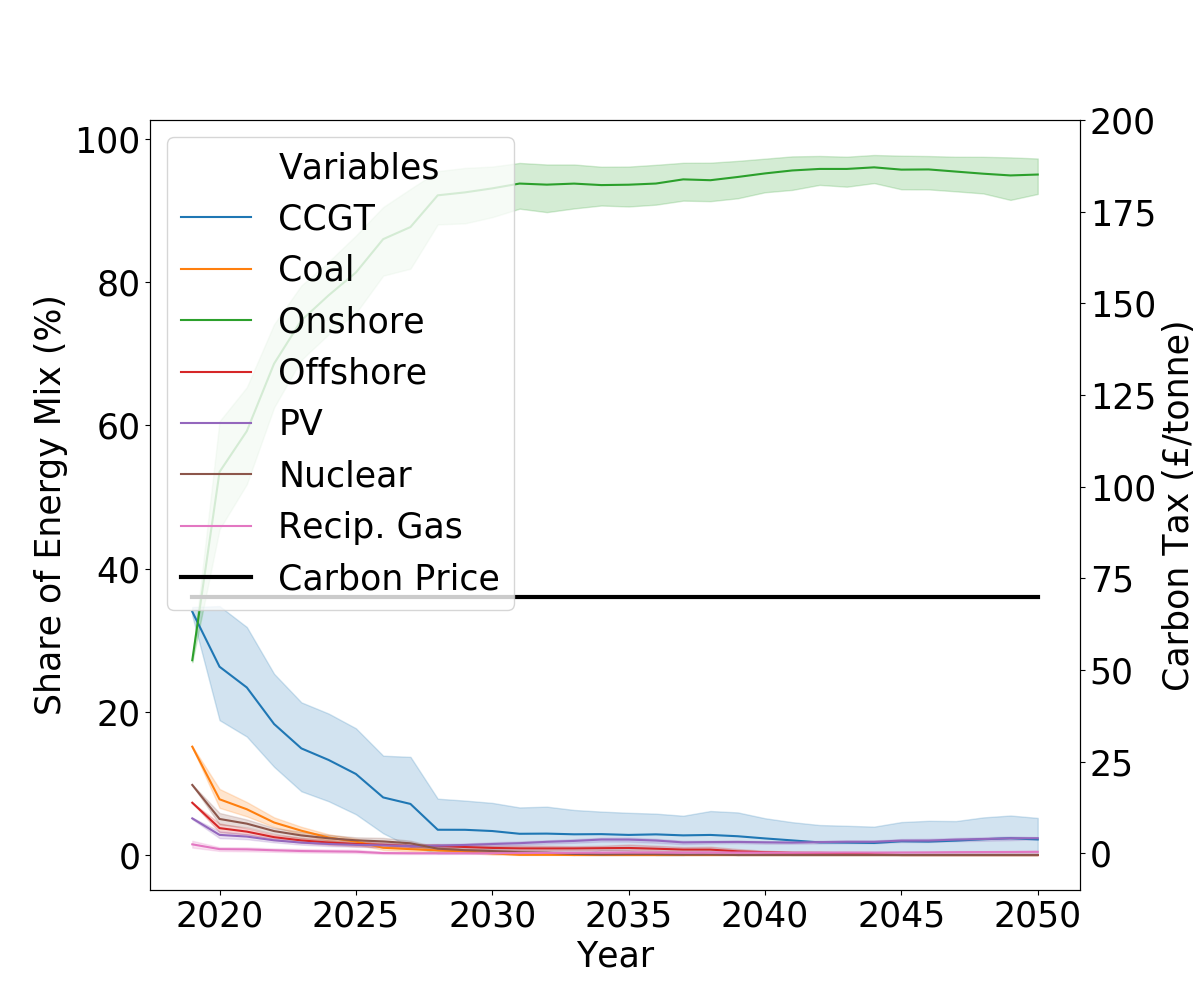
\includegraphics[width=0.5\textwidth]{figures/scenarios/demand099-carbon70-datetime.png}
		\caption{Demand decreasing by 1\% per year and a carbon tax of \textsterling20}
		\label{fig:demand99carbon70}
	\end{center}
\end{figure}



\begin{figure*}[h]
	\centering
	\begin{subfigure}[b]{0.475\textwidth}
		\centering
		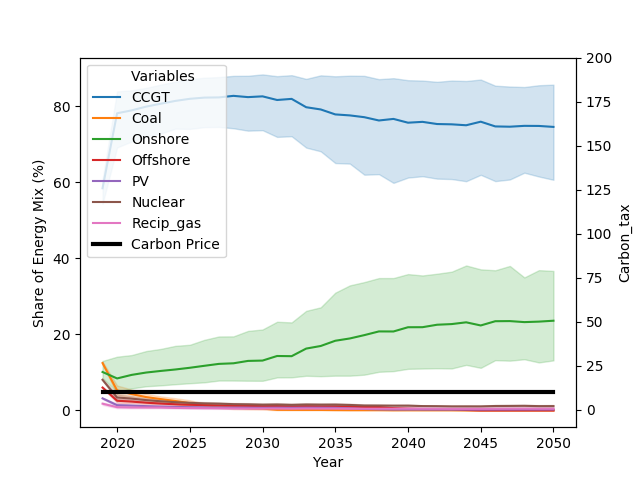
\includegraphics[width=\textwidth]{figures/scenarios/demand099-carbon10-datetime.png}
		\caption[Network2]%
		{{\small \textsterling10 carbon tax.}}    
		\label{fig:demand99carbon10}
	\end{subfigure}
	\hfill
	\begin{subfigure}[b]{0.475\textwidth}  
		\centering 
		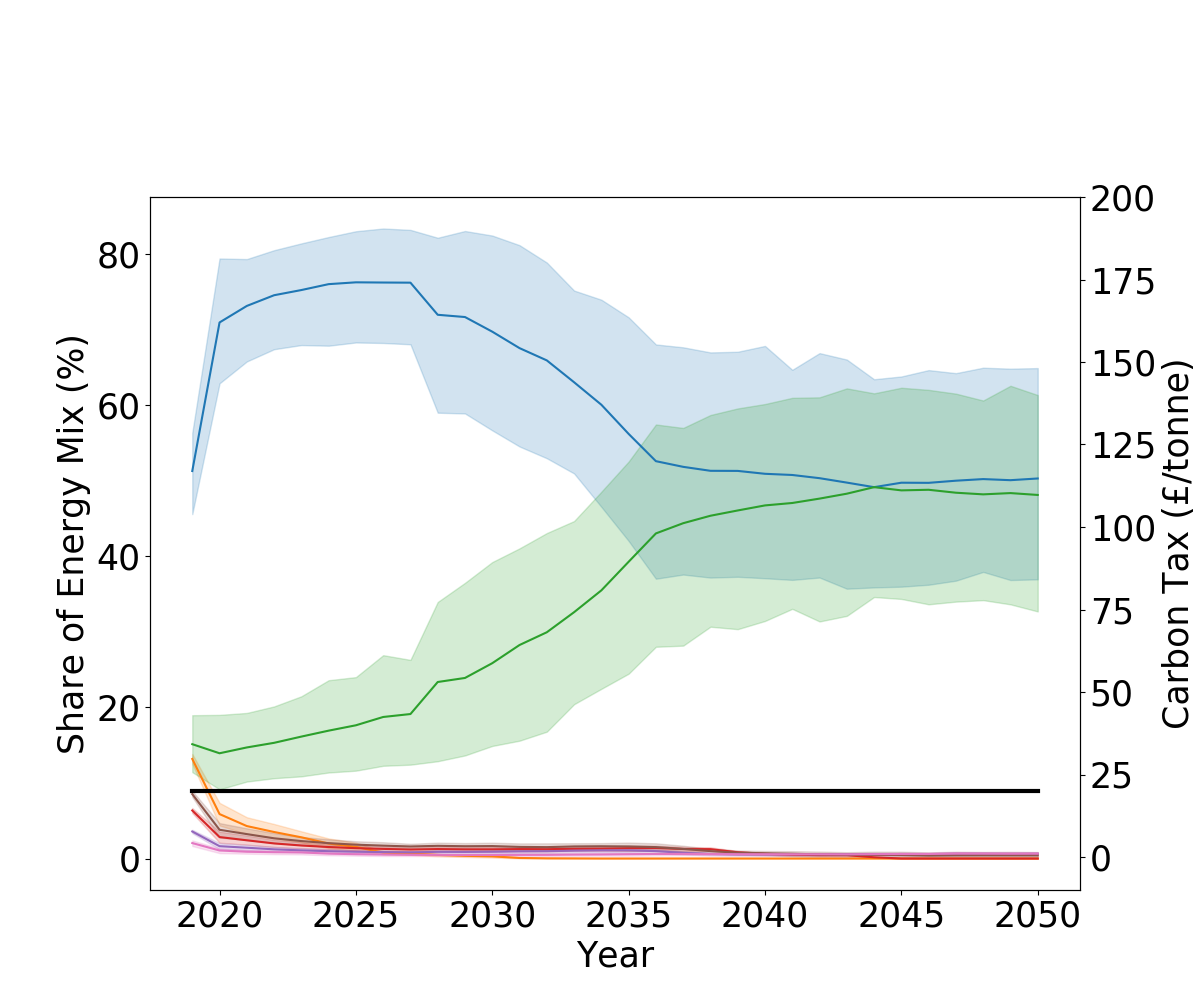
\includegraphics[width=\textwidth]{figures/scenarios/demand099-carbon20-datetime.png}
		\caption[]%
		{{\textsterling20 carbon tax.}}    
		\label{fig:demand99carbon20}
	\end{subfigure}
	\vskip\baselineskip

	\begin{subfigure}[b]{0.475\textwidth}   
		\centering 
		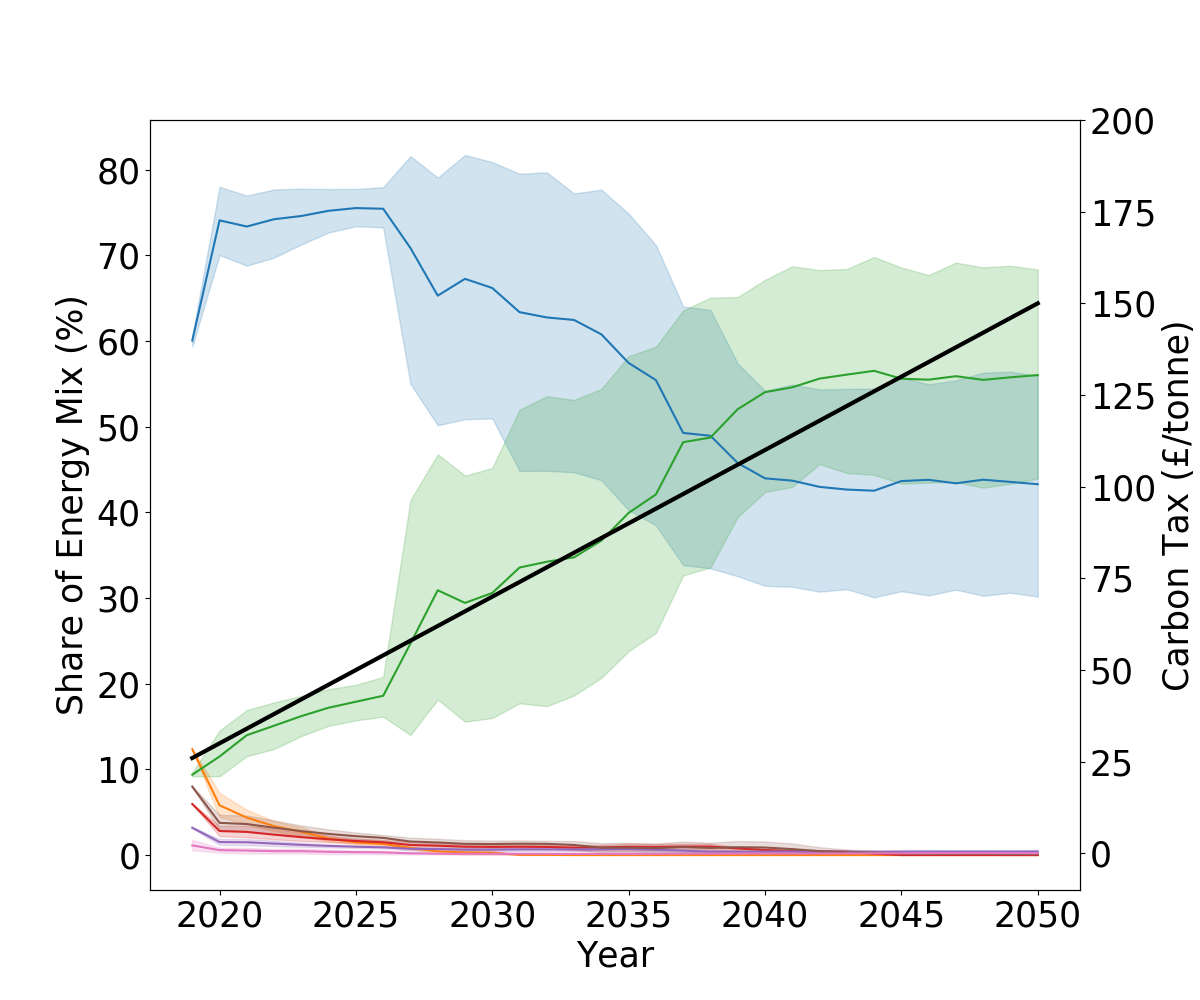
\includegraphics[width=\textwidth]{figures/scenarios/demand099-carbon18-datetime.png}
		\caption[]%
		{{\textsterling26 to \textsterling150 linearly increasing carbon tax.}}    
		\label{fig:demand99carbon18}
	\end{subfigure}
	\quad
	\begin{subfigure}[b]{0.475\textwidth}   
		\centering 
		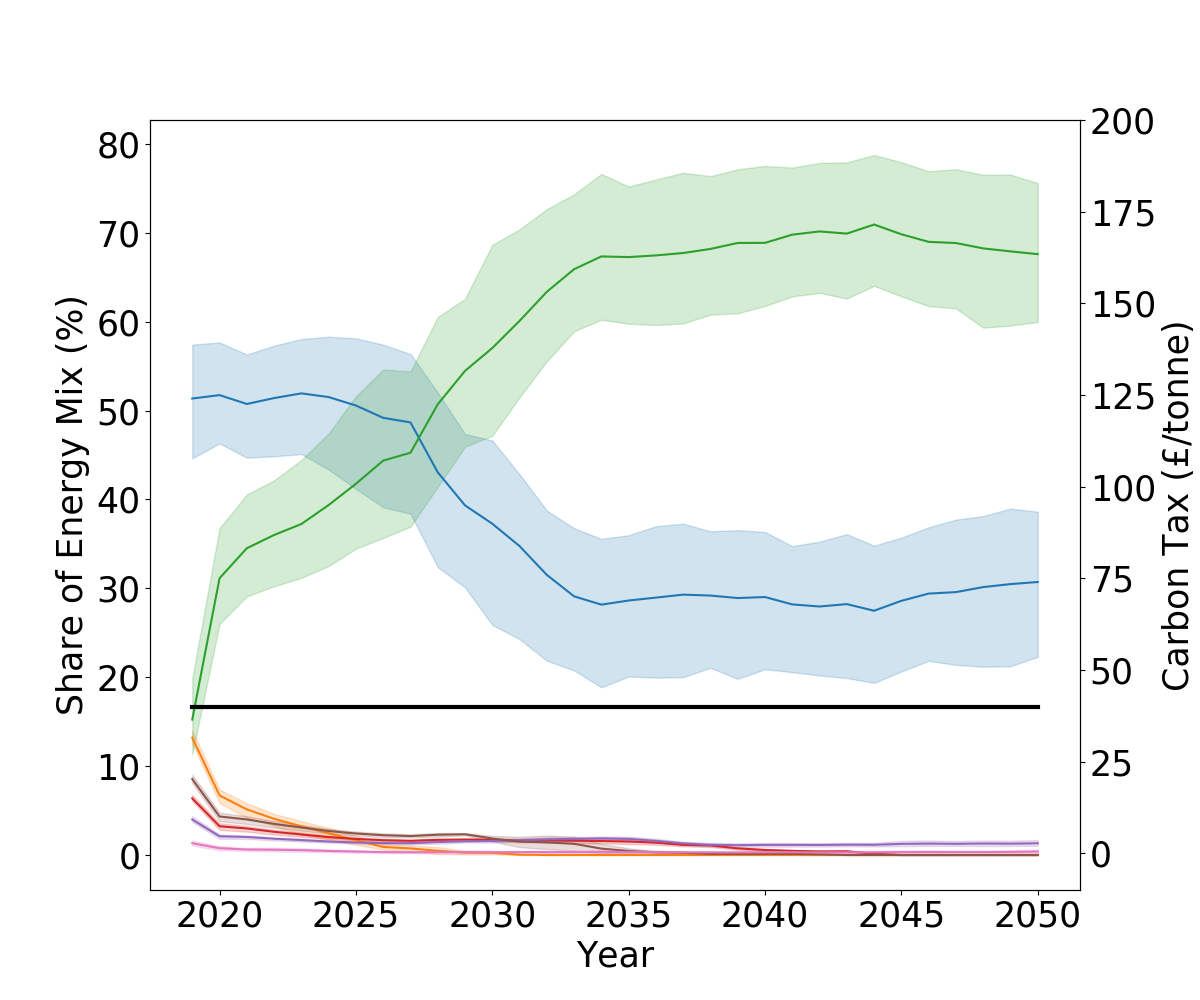
\includegraphics[width=\textwidth]{figures/scenarios/demand099-carbon40-datetime.png}
		\caption[]%
		{{\textsterling40 carbon tax.}}    
		\label{fig:demand99carbon40}
	\end{subfigure}
	\caption[ Scenarios up to the year 2050 with varying carbon taxes and decreasing demand ]
	{\small Scenarios up to the year 2050, with varying carbon taxes and electricity demand decreasing 1\% a year.} 
	\label{fig:mean and std of nets}
\end{figure*}
%\FloatBarrier








%\begin{figure}[h]
%	\begin{center}
%		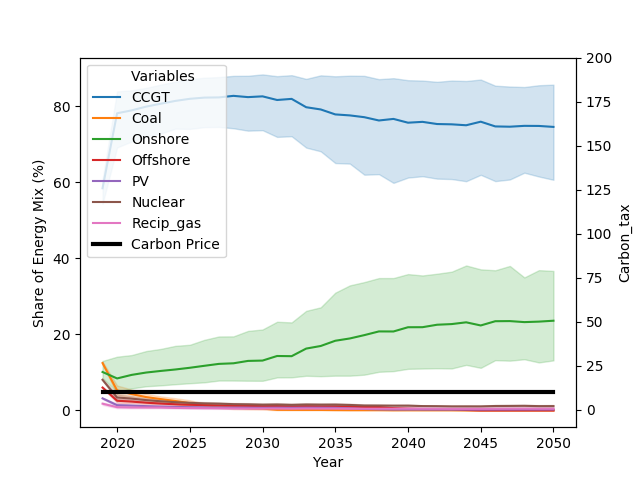
\includegraphics[width=0.5\textwidth]{figures/scenarios/demand099-carbon10-datetime.png}
%		\caption{Demand decreasing by 1\% per year and a carbon tax of \textsterling10}
%		\label{fig:demand99carbon10}
%	\end{center}
%\end{figure}
%
%\begin{figure}[h]
%	\begin{center}
%		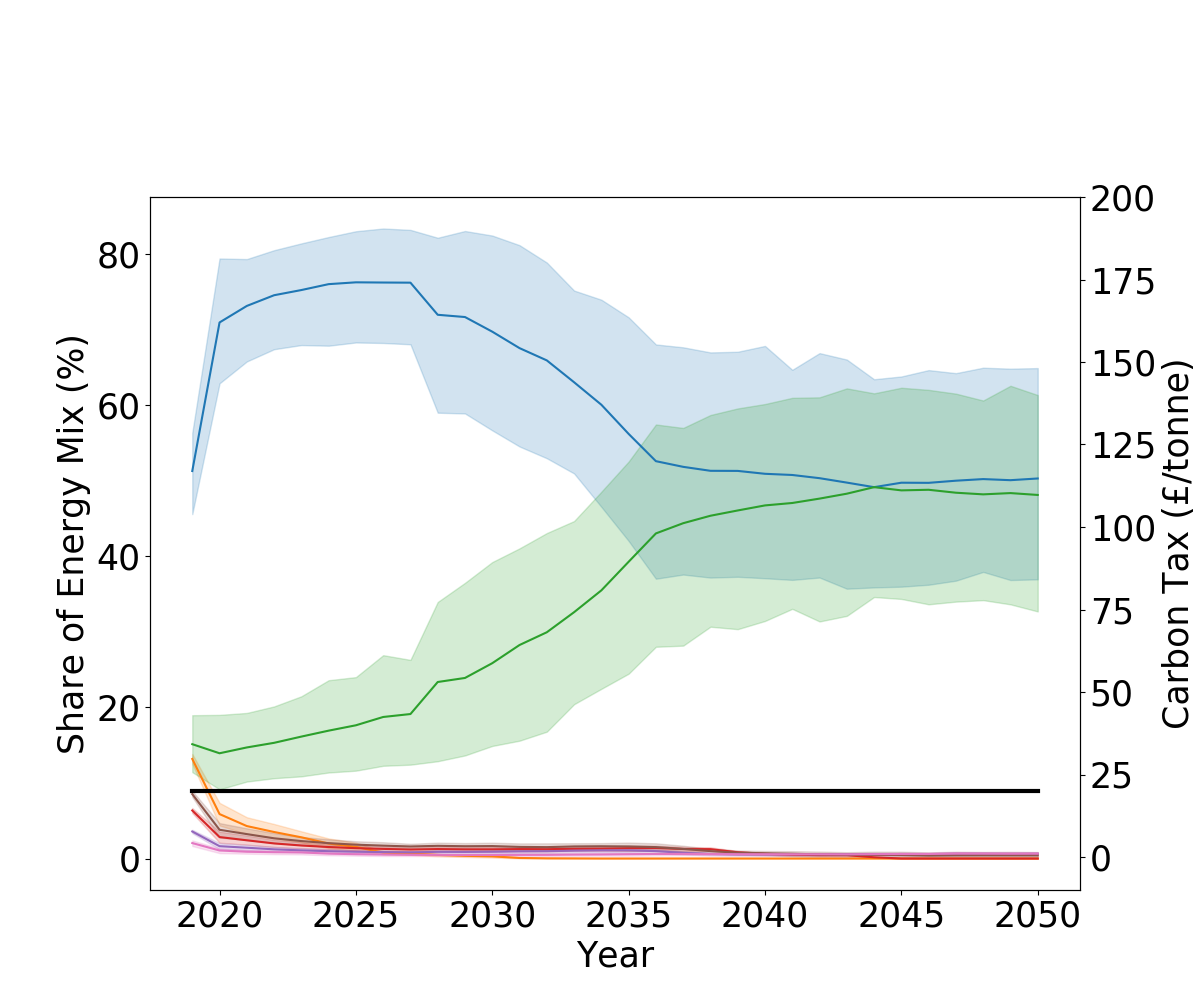
\includegraphics[width=0.5\textwidth]{figures/scenarios/demand099-carbon20-datetime.png}
%		\caption{Demand decreasing by 1\% per year and a carbon tax of \textsterling20}
%		\label{fig:demand99carbon10}
%	\end{center}
%\end{figure}
%
%
%
%\begin{figure}[h]
%	\begin{center}
%		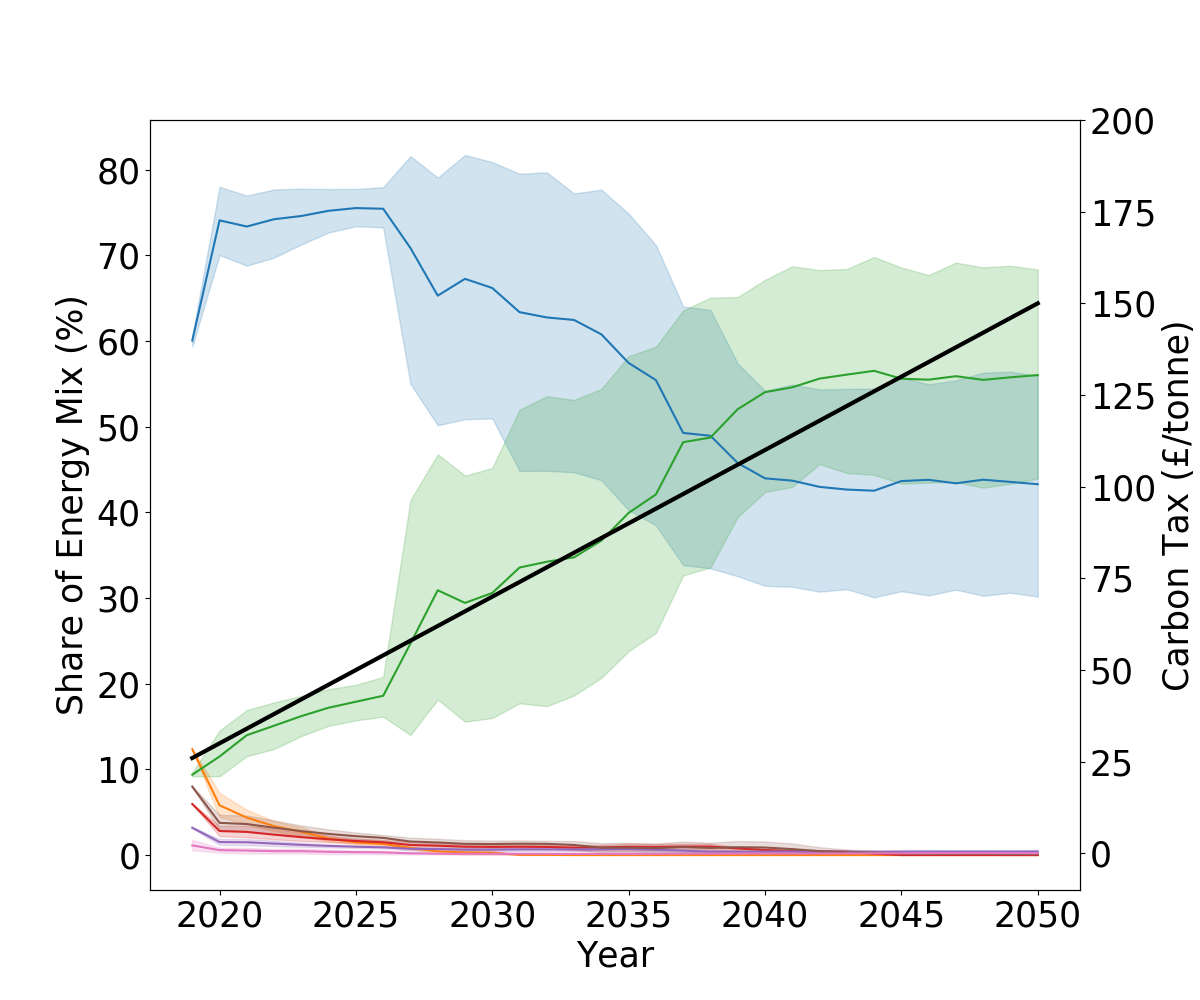
\includegraphics[width=0.5\textwidth]{figures/scenarios/demand099-carbon18-datetime.png}
%		\caption{Demand decreasing by 1\% per year and a carbon tax of \textsterling20}
%		\label{fig:demand99carbon10}
%	\end{center}
%\end{figure}
%
%
%
%\begin{figure}[h]
%	\begin{center}
%		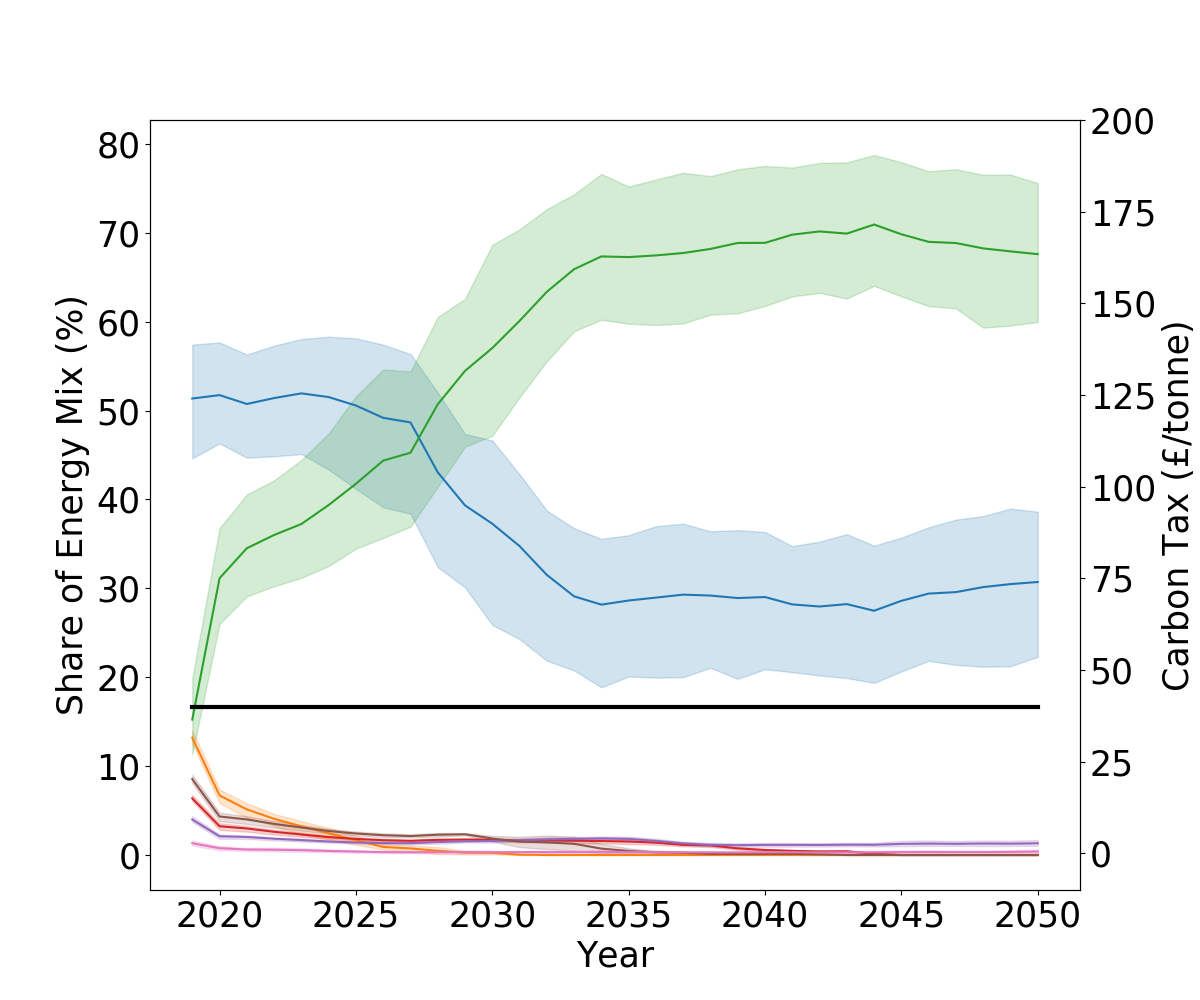
\includegraphics[width=0.5\textwidth]{figures/scenarios/demand099-carbon40-datetime.png}
%		\caption{Demand decreasing by 1\% per year and a carbon tax of \textsterling20}
%		\label{fig:demand99carbon10}
%	\end{center}
%\end{figure}











%\begin{itemize}
%	\item Effect of different carbon tax on investments made.
%	\item Effects of different demand scenarios. (High peaks, high growth, high reduction in demand)
%	\item Effects of high fuel prices.
%	\item Different costs of capital (eg. Borrowing for Nuclear of interest rate to equal 2\% at government bonds rate, as opposed to 10\% for private companies.)
%	\item Different learning rates for renewable costs.
%	\item The effect of long term carbon tax policy (eg. Carbon price known for next 25 years) vs short term changes in carbon tax.
%\end{itemize}
